\documentclass[journal, letterpaper]{IEEEtran}
\usepackage{listings}
\usepackage{fancyvrb}
\usepackage{framed}
\usepackage[listings,skins]{tcolorbox}
\usepackage[skipbelow=\topskip,skipabove=\topskip]{mdframed}
\usepackage{pbox}
\usepackage{graphicx}
\usepackage{url}
\usepackage{hyperref}
\usepackage{caption}
\linespread{1.1}
\usepackage{float}
\usepackage{tabularx} % in the preamble

\mdfsetup{roundcorner=0}
% Congyang: Added the geometry module to add the margin of bottom
\usepackage[top=1in, bottom=1.2in, left=0.7in, right=0.7in]{geometry}
% Congyang: Added the indent first module (and delete "\\" of every paragraph) to make it indent every paragraph.
\usepackage{indentfirst}

\begin{document}
\title{Highway Tollgates Traffic Flow Prediction}
\author{Congyang Wang, Fangyu Lin, Meng Li \\ Department of Computer Science, Department of Data Science -- Worcester Polytechnic Institute, MA, 01609 \\ Email: \{cwang8, flin, mli6\}@wpi.edu}
% Congyang: Added our emails
\maketitle

% The Abstract
\begin{abstract} 
\large
As urban population and economy grow, automobile penetration in urban area, especially metropolises, has increased fast. As a result, traffic congestion problem has arisen not only within cities, but also in suburb such as areas bridging highways. The highway is therefore no longer highway due to congestion. In this paper, our goal is to predict traffic volume passing through tollgates in 20-minute time interval, especially for the rush hours which are defined in 2017 KDD-CUP from 8 to 10 a.m and from 5 to 7 p.m. We are going to use Decision Tree Model, comparing with ARIMAX models to do the prediction of rush hours traffic volume by using the training dataset and testing dataset that are provided by the KDD-CUP 2017. 
\end{abstract}

% The Keywords 
\begin{IEEEkeywords}
Traffic Optimization;
Traffic Volume Optimization;
\end{IEEEkeywords}

\section{Introduction}
\large
%As the increase of population and economy, many people prefer to buy a house and live in another cities in Massachusetts. The price of apartments or houses in the cities are much more expensive than other small town, or cities. Definitely, the highway becomes the most important transportation way which connecting their homes to the working place. However, As the population increase, the number of vehicles cause the traffic congestion in the highway which makes uncomfortable to the drivers in daily life working schedule. For example, more people choose to take the Train from "Union Station" in Worcester to the "South Station" in Boston, which takes about 90 minutes (Comparing with normal average travel time 60 minutes).

Urbanization has been a global trend in recent decades, since it does not only benefit rural residents by improving accessibility of urban services and resources, the local economy also has gained momentum from the process. However, various problems have been engendered as concomitants. Inevitably, living costs surge as urban population grows and overcrowding worsens living conditions. As a consequence, a growing number of citizens choose to move to satellite towns and commute on highways. The shift in lifestyle choice intensifies pressures on highway management, since increase of traffic volume may cause congestions and lower highway performance. This, as a result, entails studies on highway traffic flows.

Highway tollgates are gateways implemented for toll collection so that highway construction costs and maintenance expenditures can be reimbursed, whereas they frequently act as blockades that cause traffic congestions, especially during rush hours and public holidays, and hence incur criticism towards the administration agency. To improve highway customer satisfaction and enhance highway performance, it is necessary to solve or at least mitigate the congestion problem caused by tollgates.  

Traffic volume prediction at tollgates enables administrators to make preparation in advance for digesting incoming high traffic volume, such as opening additional toll booths. Similarly, travel time prediction between tollgates and intersections empowers travelers to make choices over highway entrances, instead of running into dead-stop bumper-to-bumper situations unawarely. Moreover, with predicted traffic volume and travel time to a given tollgate, highway administration agency is able to regulate its upstream traffic flow to reduce chances of traffic congestions.

\section{Related Work}
\large
There is one similar research paper [3] which evaluates the electric auto-pay system and the manual pay system. As we all know that Massachusetts highway has implemented the electric auto-pay system since 1998, which is known as "E-ZPass". However, the tollgates were not removed until 2016. Then all tollgates have been removed in Massachusetts which improved the highway traffic average speed amazingly. In this paper, we assume that there is no manual tollgates at Tollgate one, two, and three for both the entry and exit direction. 

There are many good methodologies cited by other research papers. One [7] uses a loglinear model to predict the travel time in the highway. Another one [6] uses the Seasonal ARIMA Model to predict the highway volume producing more accurate results. One [4] considers the highway traffic as a multi-lane tollgates model. As we will consider the different effectiveness from the number of lanes in the tollgates, we have the data table three(links). The paper [4] considers the multi-lane as single lane to improve the average traffic velocity. Additionally, the paper [8] uses the Takagi–Sugeno–Kang Fuzzy Neural Network(TSKFNN) approach to predict the average travel time on highway and uses the back propagation neural network(BPNN) and the time series model (ARIMA) with the training trajectory data and validation trajectory data. 

\section{Methodology}
\large
\subsection{Problem Setting}
To study the efficiency of the highway traffic, we select a intersections and tollgates pairs as the target area. The Fig. \ref{fig:1} shows the detail of intersections and tollgates pairs graph. There are total six routes:

   a. Routes from Intersection A to Tollgates 2 \& 3;
   
   b. Routes from Intersection B to Tollgates 1 \& 3;
   
   c. Routes from Intersection C to Tollgates 1 \& 3.
   
\begin{figure} [H]
  \centering
  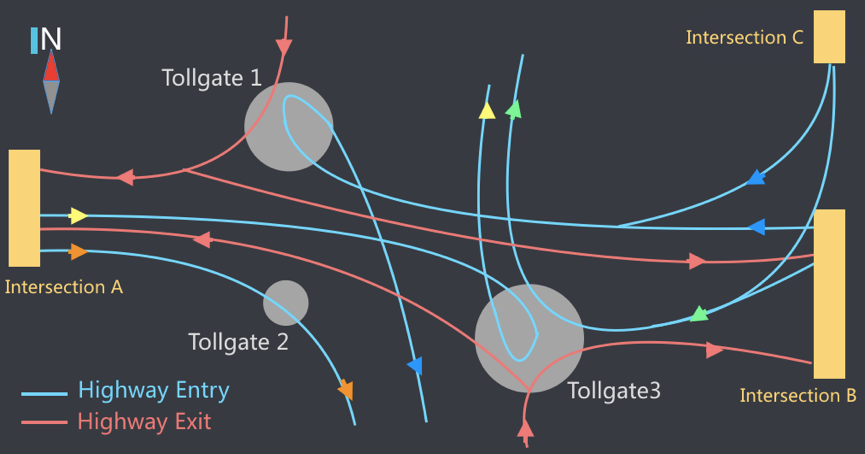
\includegraphics[width=0.48\textwidth]{road_graph.png}
  \caption{Intersection and Tollgate Network Graph}
  \label{fig:1}
\end{figure}

The road network in Fig. \ref{fig:1} here used the direction graph formed by road links with interconnected. Every route in this road network is represented by a sequence of links like the model you can see in Fig. 2.

Thee are two different tasks from KDD-CUP 2017: 

	Task 1: To estimate the average travel time from designated intersections to tollgates. 
    
    Task 2: To predict average tollgate traffic volume.

In the task 1, taking every 20-minutes as time interval, try to estimate the average travel time of vehicles for every specific route shown in Fig. 1 with our prediction models, so we will predict six average travel time for all routes. In the task 2, we will focus on the tollgate volume prediction, which takes every 20-minutes as time interval to try to predict the entry and exit of tollgate volumes at tollgates 1, 2 and 3 (tollgate 2 only has Highway Entry as shown in Fig. 1). Therefore, we need to predict the traffic volumes number for the 5 tollgate-direction pairs during the rush hours from 8 to 10 a.m and from 5 to 7 p.m.

\begin{figure} [t]
  \centering
  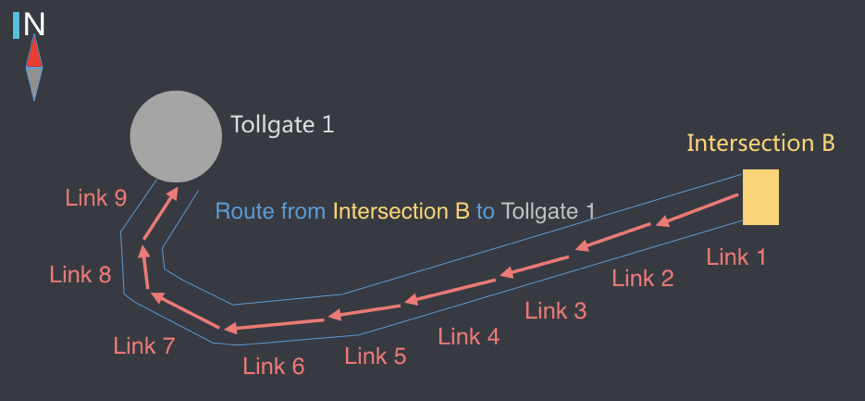
\includegraphics[width=0.48\textwidth]{link-sequence.png}
  \caption{Intersection and Tollgate Links Sequence}
  \label{fig:2}
\end{figure}

\begin{figure} [H]
  \centering
  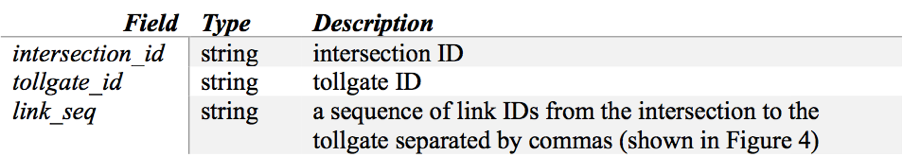
\includegraphics[width=0.48\textwidth]{route.png}
  \caption{Routes from Intersections to Tollgates}
  \label{fig:3}
\end{figure}

\subsection{Data Description}

There are five datasets which are provided from KDD-CUP 2017. Two for traffic travel time-invariable conditions, and other three are for time-variable factors. 

The invariable data table (Fig. 3) includes the link sequence from intersections to tollgates, the graph like Fig. 2, the vehicles traveling from road intersections to highway tollgates have limited options, for each intersection-tollgate pair, this dataset selected the most important one. The data table (Fig. 4) which shows more details about infrastructure design of every piece of road link, the (Fig. 5) also show the instruction of the links connection. 

For the time-variable factors like vehicle trajectories data (Fig. 6) which includes the time-stamped records of actual vehicles along the routes in (Fig. 3), traffic volume data (Fig. 7) which is the record of each vehicle pass through each tollgate from two different directions, weather data (Fig. 8) which describes the weather conditions for all the dates that are presented in Trajectories data and traffic volume record data. For more details, the traffic volume dataset contains the records from the three tollgates to entry or exit pairs. The weather data has the features which may effect the highway traffic with 3 hour time interval.

\begin{figure} [H]
  \centering
  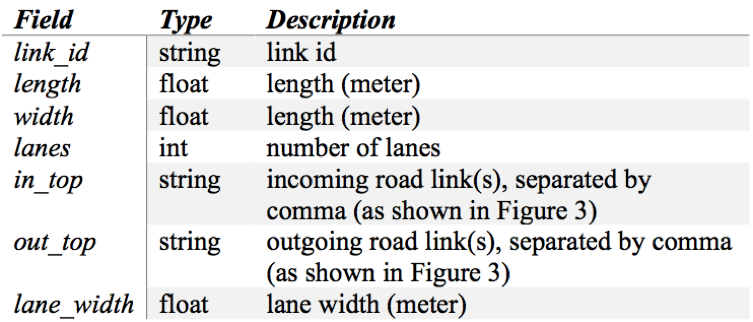
\includegraphics[width=0.48\textwidth]{road-link.png}
  \caption{Road Link Properties}
  \label{fig:4}
\end{figure}
\begin{figure} [H]
  \centering
  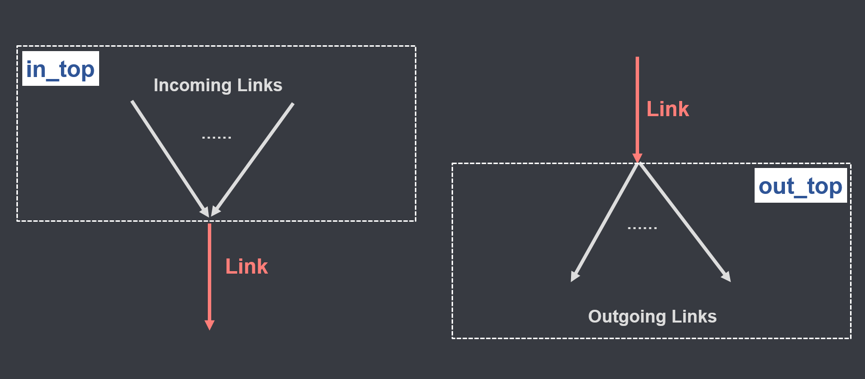
\includegraphics[width=0.48\textwidth]{in-out.png}
  \caption{Linkage In-top and Out-top Description}
  \label{fig:5}
\end{figure}

\begin{figure} [H]
  \centering
  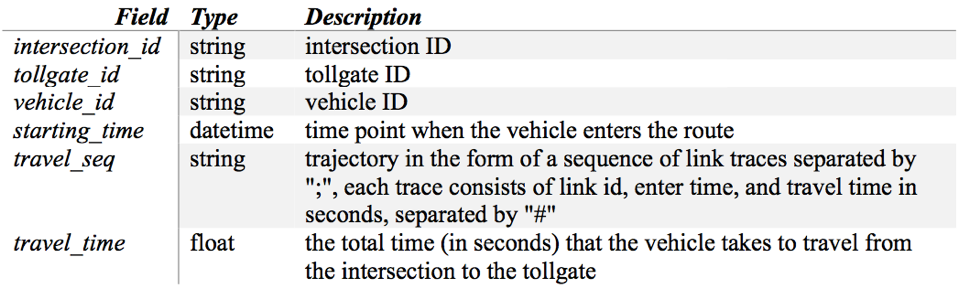
\includegraphics[width=0.48\textwidth]{trajectories.png}
  \caption{Vehicle Trajectories}
  \label{fig:6}
\end{figure}

\begin{figure} [H]
  \centering
  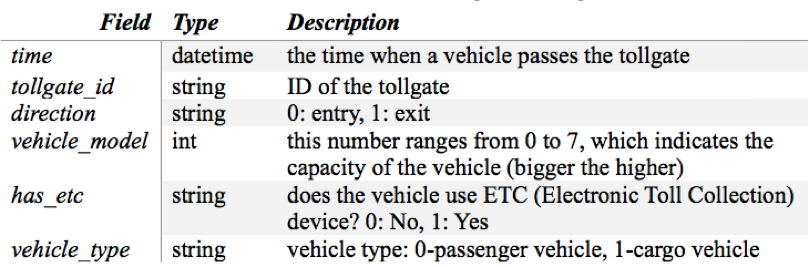
\includegraphics[width=0.48\textwidth]{volume.png}
  \caption{Traffic Volume through the Tollgates}
  \label{fig:7}
\end{figure}

\begin{figure} [H]
  \centering
  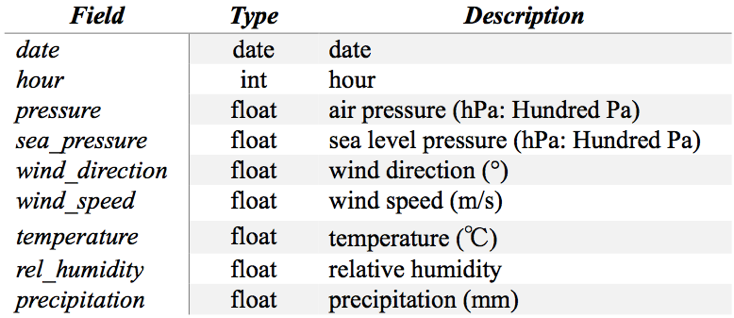
\includegraphics[width=0.48\textwidth]{weather.png}
  \caption{Weather in Target Area}
  \label{fig:8}
\end{figure}

\subsection{Preliminary Statistics}
To explore traffic volume pattern at each tollgate, the data are partitioned into uniform time slots of 20 minutes and visualized in (Fig 9).

\begin{figure} [H]
  \centering
  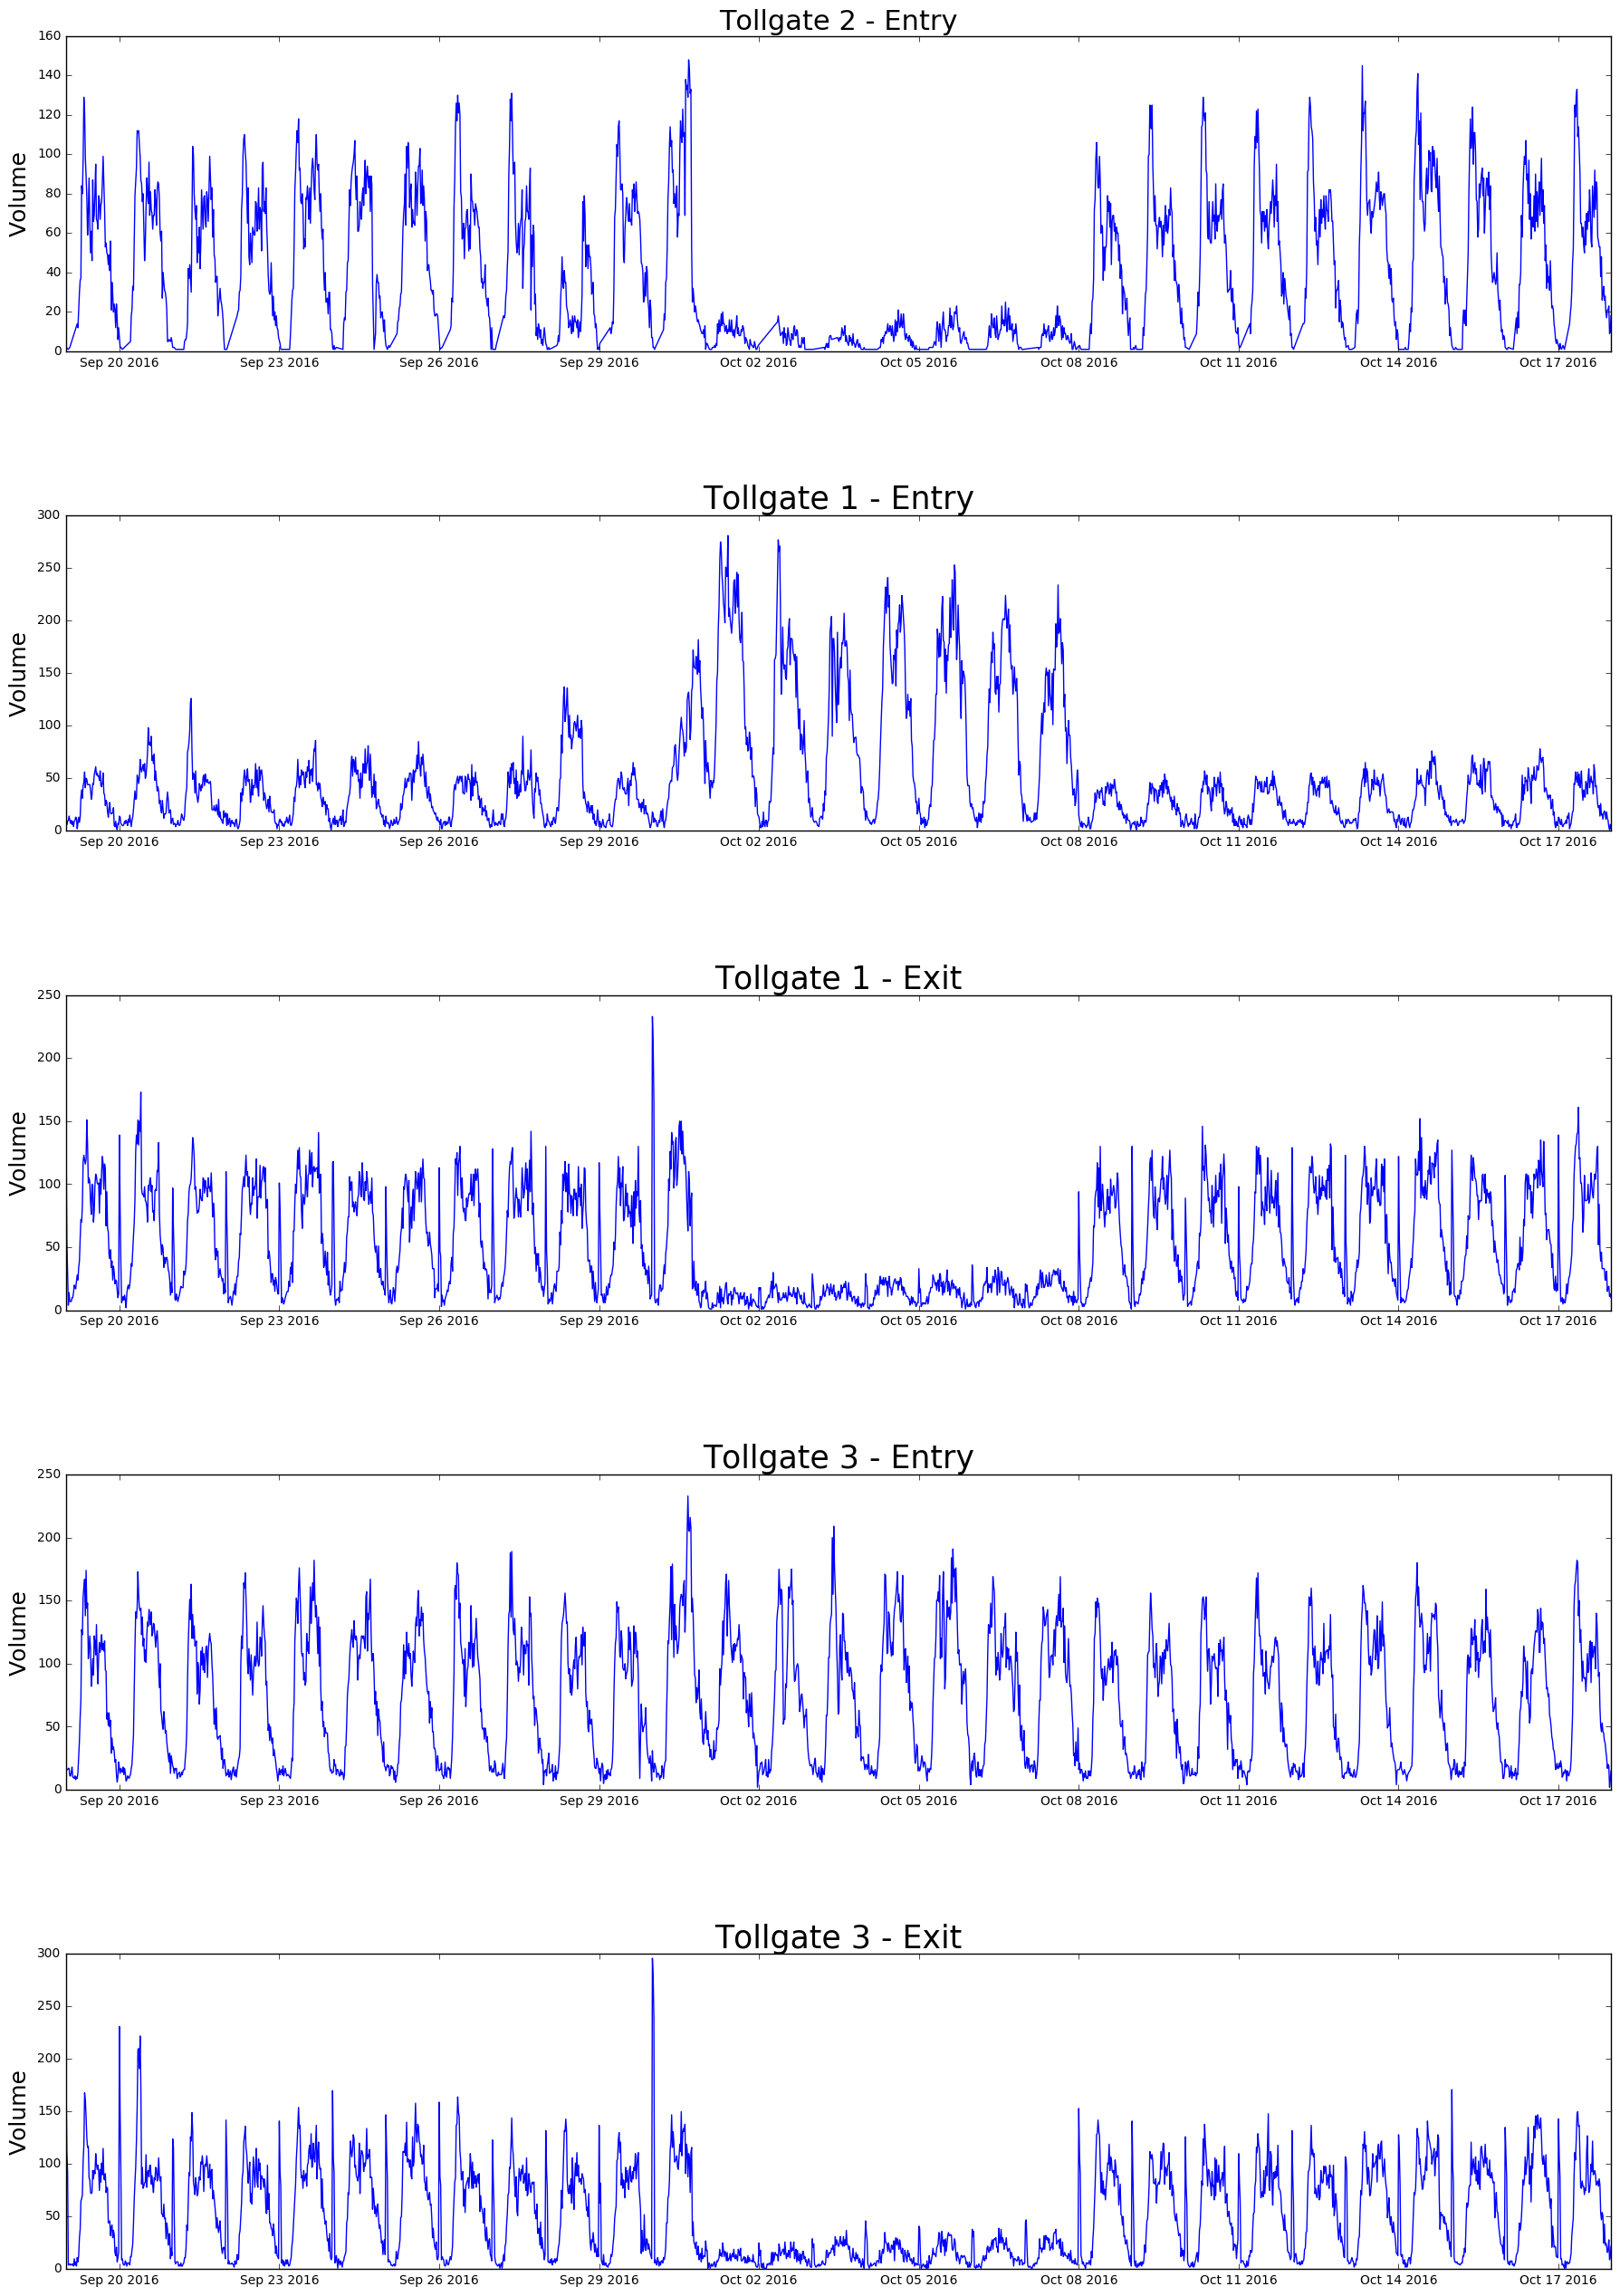
\includegraphics[width=0.35\textwidth]{tollgate-volume-3.png}
  \caption{Average Traffic Volume of Tollgate-Direction Pair Over Time}
  \captionsetup{justification=centering}
  \label{fig:9}
\end{figure}

The Fig. \ref{fig:9} shows average traffic volumes in 20-minute windows versus time for each tollgate-direction pairs, which are gate 1 entry and exit, gate 2 entry, and gate 3 entry and exit from September 19 to October 17. Apparently, average traffic volumes during October 1 to October 7 have very different patterns, compared to volumes in other time periods. The reason for these special volume patterns is that from October 1st to October 7th are Chinese National Holiday which the high way tollgates are open for all free pass. 

For every tollgate-direction pair, Tollgate1-Entry/Tollgate1-Exit/Tollgate3-Exit these 3 pairs have the similar pattern, means they may have the same characteristics we can use for the feature engineering later. The Tollgate3-Entry pair didn't show a clear affection by the national holiday. In addition, two peaks per day are observed which represent morning rush hours and afternoon rush hours traffic volume, in line with empirical observations that there are in general two rush-hour periods everyday.

\begin{figure} [H]
  \centering
  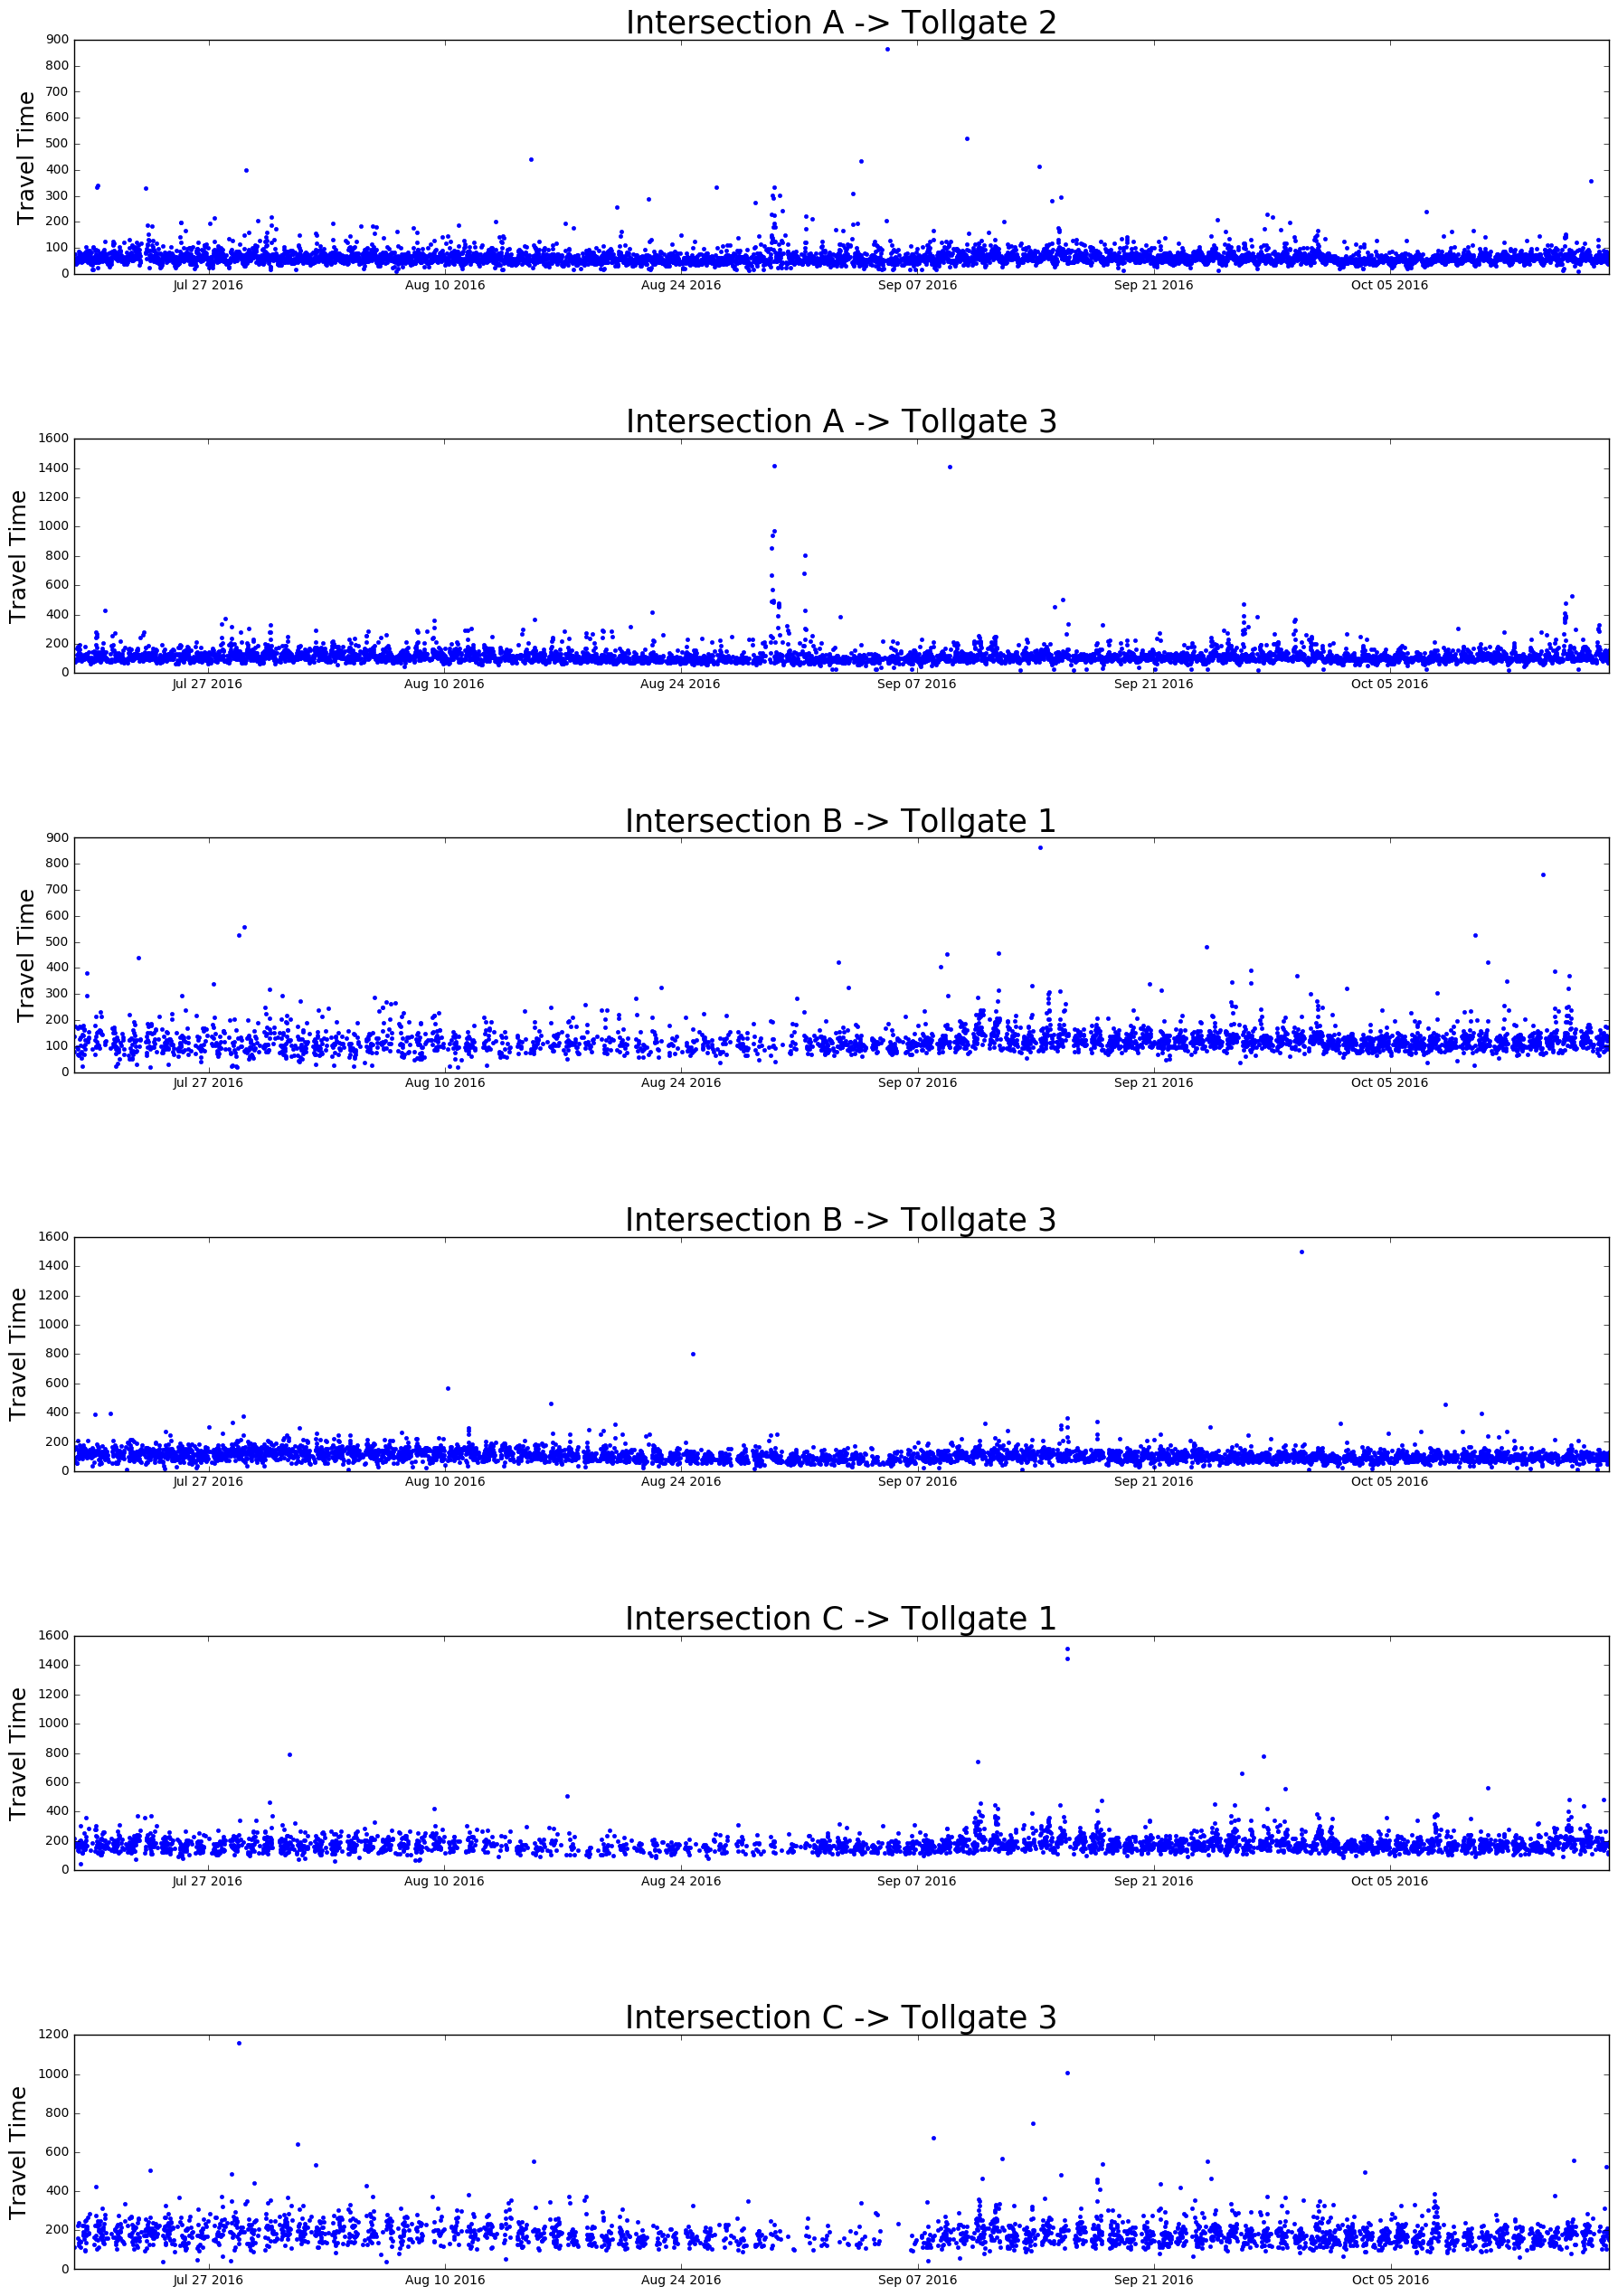
\includegraphics[width=0.35\textwidth]{intersection-tollgate-time-2.png}
  \caption{Average Travel Time from Intersections to Tollgates Over Time}
  \captionsetup{justification=centering}
  \label{fig:10}
\end{figure}

Fig. \ref{fig:10} shows average travel time in 20-minute windows from intersections to tollgates. The travel time is measured in seconds. For all intersection-tollgate pairs, the average travel time reveals a pattern that is approximately random.

To figure out reasons why a large number of anomalies appear, we took a close look at some records with high travel time. We discovered that travel time of the last link of a route, i.e., the link to tollgates, dominated the overall travel time in some cases.

Then we came up with a hypothesis that the overall travel time was impacted by traffic volume at tollgates. Specifically, when traffic volume exceeds tollgate capacity, traffic congestion will arise and consequently, overall travel time from intersections to tollgates will increase because of queuing. However, in the case where traffic volume does not reach tollgate capacity, the overall travel time is not supposed to increase as traffic volume grows.

To test the hypothesis, we plotted traffic volume versus travel time in the same time window at the same tollgate. The data records selected for the plot are those with the 10\% highest travel time from the intersection to the tollgate shown in plot titles, since tollgate capacities are unknown and it is unnecessary to put efforts into estimating them in the exploratory step. Any positive trend either linear or nonlinear will justify the hypothesis. However, Fig. \ref{fig:11} does not render any recognizable pattern, suggesting very weak relationship between traffic volume and travel time. To our surprise, high travel time appears even though traffic volume is extremely low. Therefore, the hypothesis is rejected and there must be other reasons that contribute to the anomalies and uncommon data pattern, which calls for further investigation.

\begin{figure} [H]
  \centering
  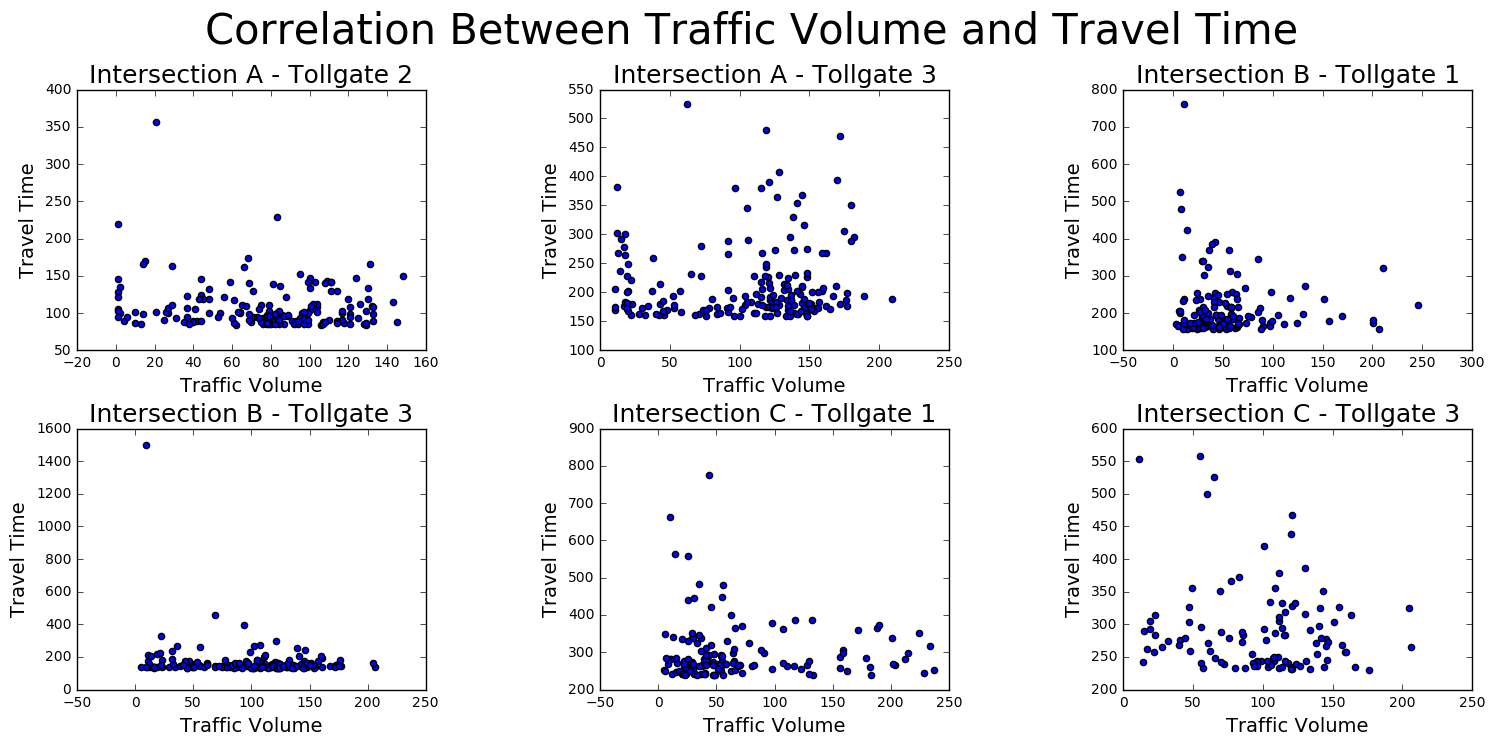
\includegraphics[width=0.48\textwidth]{corr_volume_time.png}
  \caption{Correlation Between Traffic Volume And Travel Time}
  \captionsetup{justification=centering}
  \label{fig:11}
\end{figure}

\subsection{First Approach}
As we have read previous KDD-CUP research paper, there are some tricky approach to start the prediction. The most common way is to use the average value as the predicted value, or use the Medium value for prediction.
\subsubsection{All data:}
We are going to use all the dataset from September 19 to October 17, and all 24 hours time intervals from the dataset that described in (Fig. 7) as input to calculate the average volume for prediction of each 20 minutes time interval during rush hours 8 to 10 a.m and 5 to 7 p.m from October 18 to October 24. 
\subsubsection{Remove Holiday:}
As previous data visualization and plots, we have identify the special noise of data pattern during the holiday. In this case, we decide to remove the 7 days national holiday from the dataset and calculate the average volume for October 18 to October 24 volume prediction.
\subsubsection{Rush Hours Only:}
For a better test result, we find out that the rush hours have much larger traffic volume than other time interval. In this case, we assume that other time interval have less effect to the rush hours. So we decide to remove other time interval except the rush hours to calculate the average volume for each 20 minutes time interval from 8 to 10 a.m and 5 to 7 p.m. Furthermore, we have proposed the day of week mapping methods for the average volume prediction. The idea is to classify through Monday to Sunday, and calculate the average traffic volume for each day and map it to October 18-24 week of 7 days. The proposed mapping model has three levels of group by. First level is identified as the day of week. Second level is called tollgate number and entry, exit pairs. The third level is identified as 20 minutes time interval from 8 to 10 a.m and 5 to 7 p.m. which contains total 12 time slots per day per tollgate pairs. 

\subsection{Decision Tree Approach}
The reason we choose the decision tree model is that it is a good fit for the numerical prediction, which matches the volume number in 20 minutes time interval. The prediction result has 420 list of volume numbers according to the tollgates entry and exit pairs, and 12 time intervals per day for October 18 to October 24. It is also a fast running model for large training dataset and testing dataset prediction. 
\subsubsection{Variable Definition}
Variable 'X' is defined as input training variable, which is the list of volume numbers according to 20 minutes time interval 6 to 8 a.m and 3 to 5 p.m. Variable 'Y' is defined as a list of predicted time interval from 8 to 10 a.m and 5 to 7 p.m. The detail of time interval is shown in (Fig. 12) in the experiment section. 
\subsubsection{Parameter Estimation}
First, we have realize that the holiday has different volume patterns than normal days so we remove the 7 days holiday data from October 1 to October 7. 
Second, we follow the first approach to remove other time intervals except the rush hours as the training data input. There are total 8 hours, from 6 to 10 a.m and 3 to 7 p.m, and split to X and Y accordingly as 4 hours each as input values for Decision Tree. 
Third, we use cross validation method which define the 'K' equals to 6 folds. It means that we will use the first fold for testing, and the other 5 folds for the training. 
Forth, we use the evaluation function to calculate find out the smallest MAPE by selecting different folds for the training and testing set. And pick the decision tree model with the smallest MAPE value for the prediction. 
Fifth, apply the new testing set from KDD-CUP, which only has the time interval from 6 to 8 a.m and from 3 to 5 p.m as the 'X', and we are going to get the 'Y' value from time interval 8 to 10 a.m and from 5 to 7 p.m. In this case, we are no able to validate the predicted volume numbers because there is no ground truth. The only way is upload the predicted values to KDD-CUP and find out the MAPE result which is calculated by the Organizer, who holds the real ground truth. 

\subsection{ARIMAX Approach}
\subsubsection{Fourier Transformation}
We are going to apply the Fourier Transformation function to the traffic volume data from KDD-CUP. The goal is to find out the frequency of repeating cycles. The input values to the fourier transformaiton function is the volume number in 20 minutes time interval from September 18 to October 17. We did not remove the holiday data becuase it have no effect to find the right frequency cycles. The Fourier Transformaition function will take the input traffic volume nubmer as a list of signals and decompose it to some kind of musical chord in the right peaches. The Fourier function is describe as below:
$$e^{2\pi i \theta} = cos(2\pi\theta) + i*sin(2\pi\theta)$$
We replace the variable $\theta$ with a list of the traffic volume numbers to generate a sequence of value and find out the frequency of traffice volume. The reason why we need to know the frequency of traffic volume is that it can help us using the ARIMAX model. Another purpose of using the Fourier Transformation is to make a guess of frequency and use it as a variable to improve the prediction accuracy of ARIMAX Model. The advantage of using the Fourier Transformaiton is to let data speak by itself, which means unsupervised learning is more useful than supervised learning in our case. 
\subsubsection{Features Selection}
After we have done the fourier transformation, we are going to use the frequency as a new feature selection. We know the repeat cycle of 20 minitues time intervals which define as $X_{1}$, $X_{2}$,...$X_{5}$ features for daily. The function we proposed for the ARIMAX is shown as the follow:
$$Y_{t} = \sum_{i=1}^{p}\varphi_{i}Y_{t-1}+\sum_{j=1}^{q}\theta_{j}Y_{t-1}+\sum_{k=1}^{5}\beta_{k}X_{k} +\varepsilon $$
We will assign different weights for different five features we have randomly selected from the the Fourier Transformation to the ARIMAX model function. As we know from the ARIMAX function that it will run in the iterative way because it follows the time series. The variable $\varphi$ is the weight for the prious frequency cycle. The variable $\theta$ is the weight for another frequency cycle. And the $\beta$ is the weight for different five features we have choosen. 

\section{Experiments}
\large
%aa\\
The data we use to do the experiment is from "KDD CUP 2017" traffic Volume data. In this section, we are going to focus the rush hours traffic volume prediction for each tollgate entry and exit pairs. Define the time interval T is from 6:00 to 8:00 a.m. and from 5:00 to 7:00 p.m. as input training data as X values. The Y value time interval T is from 8:00 to 10:00 a.m. and from 7:00 to 9:00 p.m. as input training data. The training date is from Sep.19 to Oct.17 to train the model. The validation data set is from Oct.18 to Oct.24 which is one week to predict the rush hours traffic volume in the same time interval, which shows the Time Window in Figure\ref{fig:12}. 

In the following sections, Section A shows the first round with the mean value of the five pairs individually. Section B shows the second round attempts the decision tree model. Section C shows the third attempts with the time series model ARIMAX. The result table is too big so we are going to plot them as continue lines.

\begin{figure} [H]
  \centering
  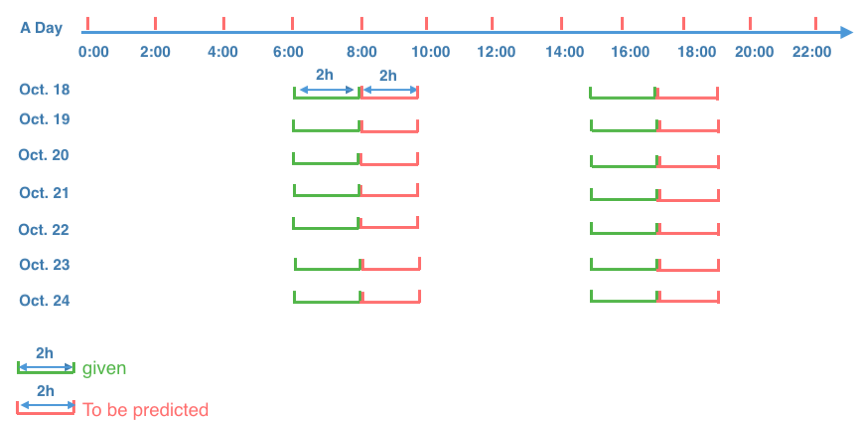
\includegraphics[width=0.48\textwidth]{time-window.png}
  \caption{Time Window}
  \captionsetup{justification=centering}
  \label{fig:12}
\end{figure}

\subsection{Mean Value Approach}
\subsubsection{All data}
We use all the training dataset from September 19 to October 17 and count the traffic volume as 20 minutes time interval. Calculate the average volume for according time interval from October 18 to October 24. The result template table is in (Fig. 13). The result of MAPE evaluated from the KDD-CUP organization is 0.441 with rank of 36 in that day. We found out that the pattern is too flat at the peak time, and the traffic volume number looks flat for all the three tollgates. We guess that this prediction result is less fitting than the true volume numbers. 
\begin{figure} [H]
  \centering
  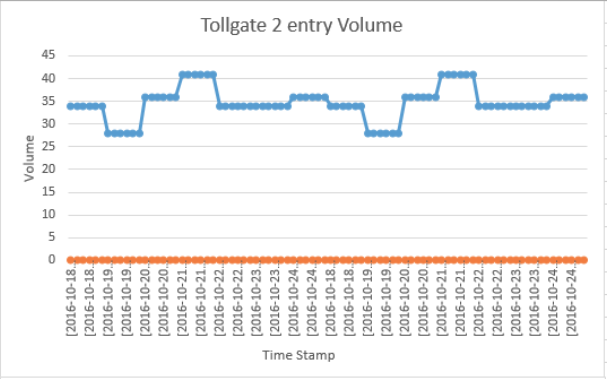
\includegraphics[width=0.48\textwidth]{t2_1.png}
  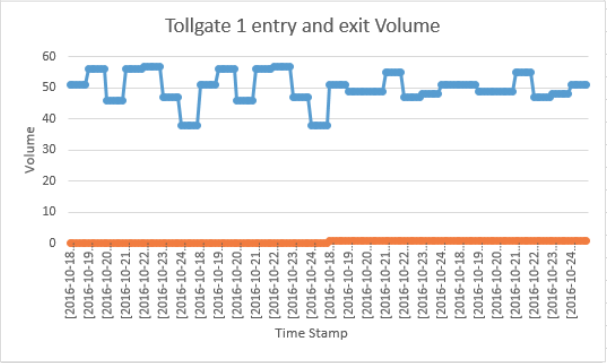
\includegraphics[width=0.48\textwidth]{t1_1.png}
  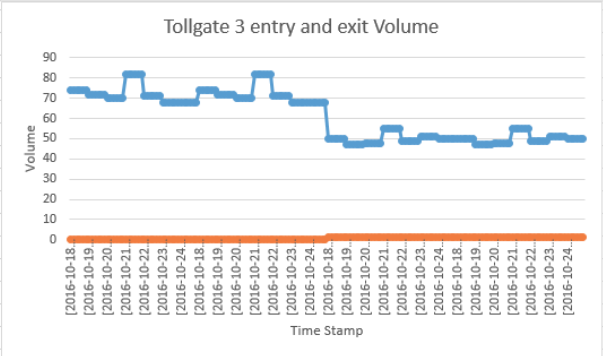
\includegraphics[width=0.48\textwidth]{t3_1.png}
  \caption{Volume Prediction Result 1}
  \label{fig:13}
\end{figure}

\subsubsection{Remove Holiday}
We remove the holiday dataset which is from October 1 to October 7. And still use the same average volume calculation to the prediction values from October 18 to October 24. Amazingly, the result looks much better than the previous flat pattern. The result of MAPE from KDD-CUP organizer is 0.336 with daily ranking 49 which is better than the previous results. From the result pattern, we assume that the pattern is over fitting. We can see in (Fig. 14)

\begin{figure} [H]
  \centering
  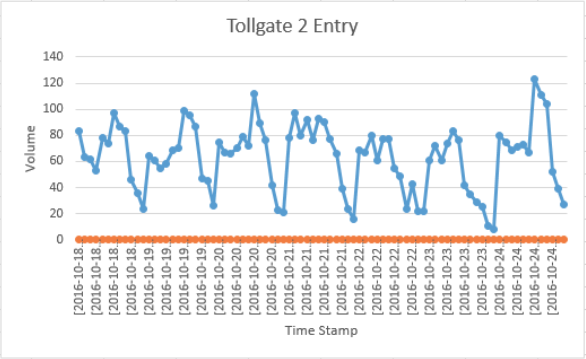
\includegraphics[width=0.48\textwidth]{t2_2.png}
  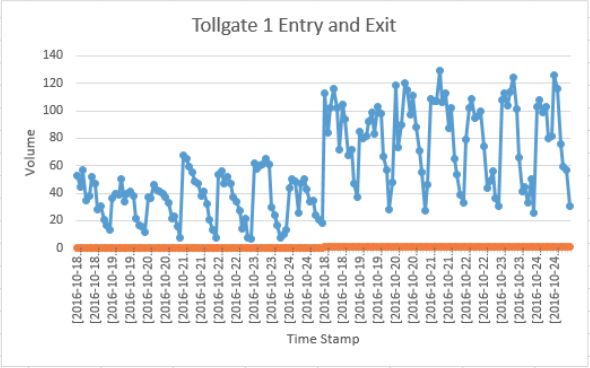
\includegraphics[width=0.48\textwidth]{t1_2.png}
  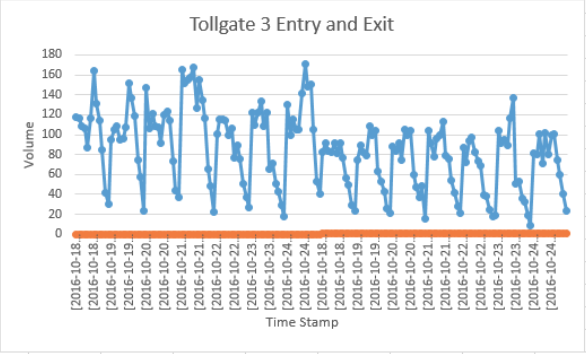
\includegraphics[width=0.48\textwidth]{t3_2.png}
  \caption{Volume Prediction Result 2}
  \label{fig:14}
\end{figure}

\subsubsection{Only rush hours}
We remove all other time interval except 8 rush hours. We propose the day of week mapping model to calculate each day and each time intervals. For example, October 19 is Monday so we calculate average volume of all the Monday time interval for the prediction result for each tollgate entry and exit. We found out that the weekends and weekdays have very big effect to each other.By using this mapping model, we get the MAPE result from KDD-CUP 0.191 with daily rank 56 total. From the (Fig. 15) we can see that these pattern is quite similar than previous results only remove the holidays. However, the new volume patterns tell us that this may reduce the over fitting from the previous result from experience. 

\begin{figure} [H]
  \centering
  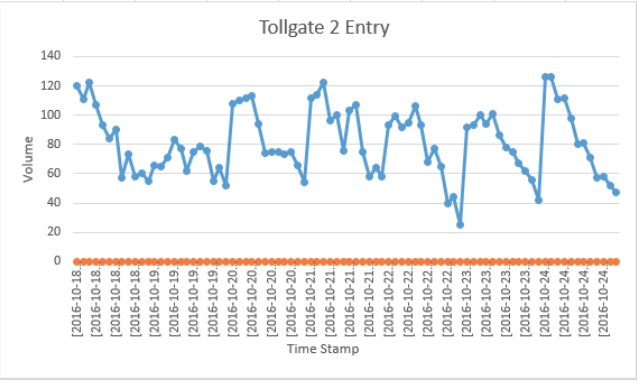
\includegraphics[width=0.48\textwidth]{t2_3.png}
  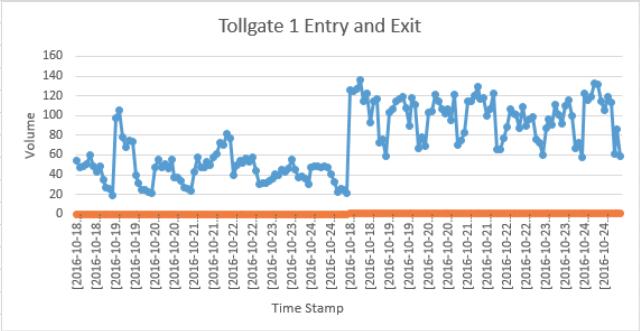
\includegraphics[width=0.48\textwidth]{t1_3.png}
  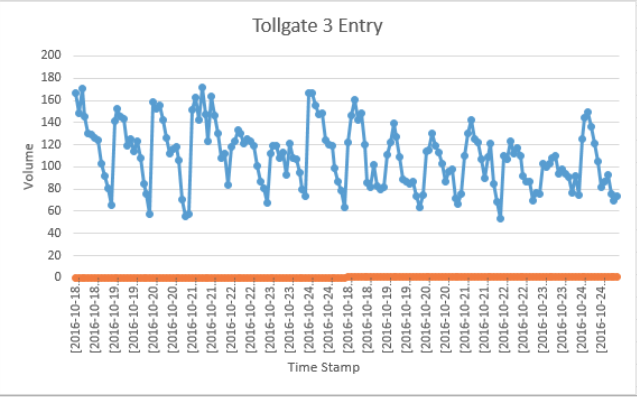
\includegraphics[width=0.48\textwidth]{t3_3.png}
  \caption{Volume Prediction Result 3}
  \label{fig:15}
\end{figure}

\subsection{Decision Tree Result}
The optimal values of the min\_sample\_split, i.e., minimum number of samples required to split internal nodes, for each decision tree is given below,

\begin{table}[ht]
%\caption{} % title of Table
\centering % used for centering table
\begin{tabular}{c |c |c |c |c} % centered columns (4 columns)
\hline\hline %inserts double horizontal lines
TollgateID & Direction & Time & min\_sample\_slt & Avg MAPE \\ % inserts table
%heading
\hline % inserts single horizontal line
1 & Entry & 08:00-10:00 & 111 & 0.172 \\ % inserting body of the table
\hline
1 & Entry & 17:00-19:00 & 71 & 0.261 \\
\hline
1 & Exit & 08:00-10:00 & 111 & 0.146 \\
\hline
1 & Exit & 17:00-19:00 & 111 & 0.287 \\
\hline
2 & Entry & 08:00-10:00 & 111 & 0.289 \\ 
\hline
2 & Entry & 17:00-19:00 & 51 & 0.235 \\
\hline
3 & Entry & 08:00-10:00 & 99 & 0.144 \\ 
\hline
3 & Entry & 17:00-19:00 & 17 & 0.275 \\
\hline
3 & Exit & 08:00-10:00 & 85 & 0.147 \\
\hline
3 & Exit & 17:00-19:00 & 111 & 0.187 \\
\hline %inserts single line
\end{tabular}
\label{table:nonlin} % is used to refer this table in the text
\end{table}

The overall MAPE reported by KDD CUP is $0.2298$.

\subsection{ARIMAX Result}
The graph below plots log-transformed (base $10$) power spectrum vs. frequencies, after applying Fourier Transform on the whole training dataset. The cycles corresponding to the top 10 frequencies, are given in the table.

\begin{figure} [H]
  \centering
  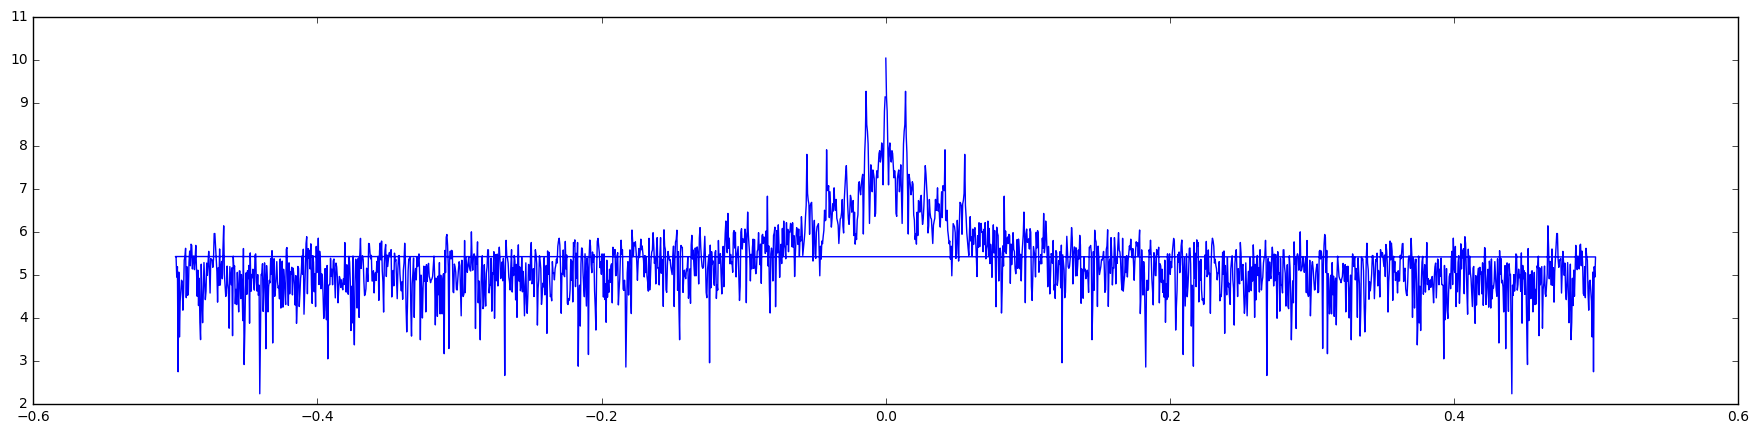
\includegraphics[width=0.48\textwidth]{FT.png}
  \caption{Log-transformed Power Spectrum vs. Frequency of Training Data}
  \label{fig:16}
\end{figure}

\begin{table}[ht]
%\caption{} % title of Table
\centering % used for centering table
\begin{tabular}{c| c| c } % centered columns (4 columns)
\hline\hline %inserts double horizontal lines
Frequency & Cycle & Approx.Cycle \\ % inserts table
%heading
\hline % inserts single horizontal line
0 & $\inf$ & $\inf$ \\
\hline
0.013889 & 72 & One Day   \\ % inserting body of the table
\hline
0.000479 & 2088 & 29 Days (the whole training data) \\
\hline
0.000958 & 1044 & 14 Days (half the training data) \\
\hline
0.013410 & 74.57 & One Day and $40$ minutes\\
\hline
0.012931 & 77.33 & One Day and $1$ hour and $40$ minutes \\
\hline
0.012452 & 80.31 & One Day and $2$ hour and $40$ minutes \\
\hline
0.014368 & 69.6 & $23$ hours \\
\hline
0.041667 & 24 &  $8$ hours\\
\hline
0.001437 & 696 & $10$ Days \\
%4 & 3 & $Y_{i} \sim Y_{i-18} + Y_{i-24}$ & 0.295  \\
\hline %inserts single line
\end{tabular}
\label{table:nonlin} % is used to refer this table in the text
\end{table}

The graph shows the log-transformed power spectrum vs. frequency of traffic volume on September $19$, $2016$. Cycles corresponding to the top $6$ frequencies are summarized in the table below.

\begin{figure} [H]
  \centering
  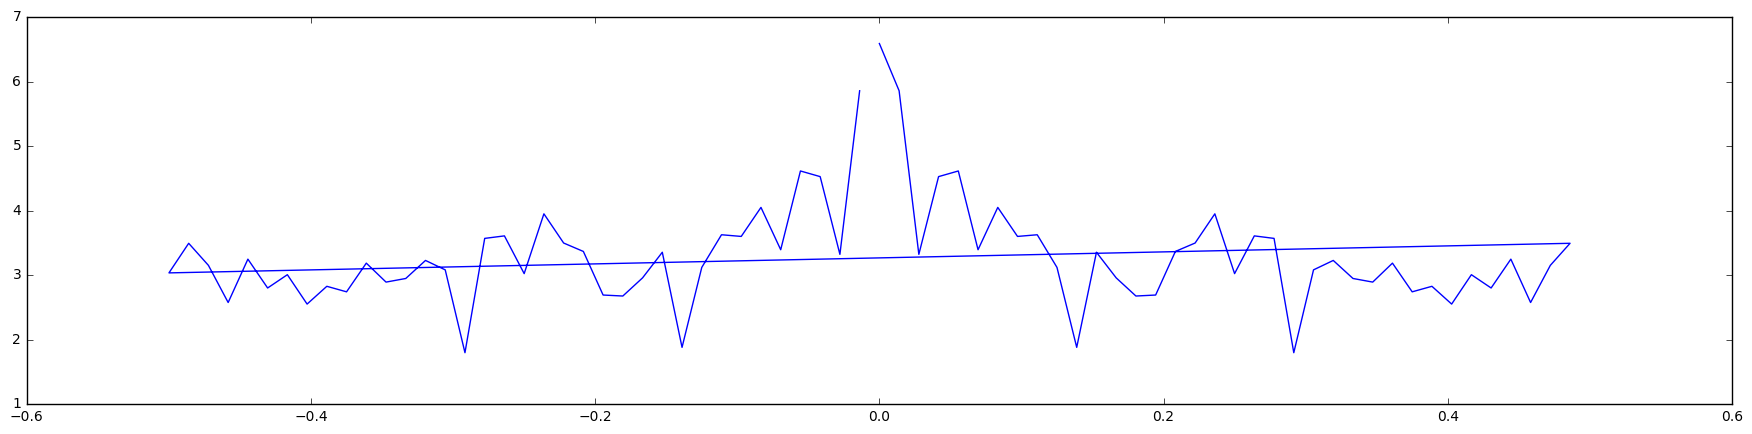
\includegraphics[width=0.48\textwidth]{ft_oneday.png}
  \caption{Log-transformed Power Spectrum vs. Frequency of Sep. $19$, $2016$}
  \label{fig:17}
\end{figure}

\begin{table}[ht]
%\caption{} % title of Table
\centering % used for centering table
\begin{tabular}{c| c| c } % centered columns (4 columns)
\hline\hline %inserts double horizontal lines
Frequency & Cycle & Approx.Cycle \\ % inserts table
%heading
\hline % inserts single horizontal line
0 & $\inf$ & $\inf$ \\
\hline
0.013889 & 72 & One Day   \\ % inserting body of the table
\hline
0.041667 & 24 & $8$ hours \\
\hline
0.055556 & 18 & $6$ hours \\
\hline
0.097222 & 10.29 & $3.5$ hours\\
\hline
0.111111 & 9 & $3$ hours \\
\hline
%4 & 3 & $Y_{i} \sim Y_{i-18} + Y_{i-24}$ & 0.295  \\
\hline %inserts single line
\end{tabular}
\label{table:nonlin} % is used to refer this table in the text
\end{table}

Based on the table, we select volumes $8$ hours ahead, volumes $6$ hours ahead, and volumes $3$ hours ahead as features. Since our previous study indicated that adding daily maximum volume could increase prediction accuracy, the daily maximum volume is also selected as one feature.\\ 

The following table shows the top $10$ models that produce the $10$ smallest mape values on volumes during $06:00-08:00$ and $15:00-17:00$ in the test phase 1 data.

\begin{table}[ht]
%\caption{} % title of Table
\centering % used for centering table
\begin{tabular}{c| c| c| c } % centered columns (4 columns)
\hline\hline %inserts double horizontal lines
p & q & Linear Model & MAPE \\ % inserts table
%heading
\hline % inserts single horizontal line
6 & 3 & $Y_{i} \sim max_{daily}$ & 0.286 \\
\hline
5 & 8 & $Y_{i} \sim max_{daily} + Y_{i-9} + Y_{i-24}$ & 0.288  \\ % inserting body of the table
\hline
12 & 6 & $Y_{i} \sim max_{daily}$ & 0.290 \\
\hline
6 & 5 & $Y_{i} \sim max_{daily} + Y_{i-9} + Y_{i-24}$ & 0.290 \\
\hline
10 & 4 & $Y_{i} \sim max_{daily} + Y_{i-9} + Y_{i-18}$ & 0.291  \\
\hline
7 & 10 & $Y_{i} \sim max_{daily} + Y_{i-18}$ & 0.291 \\
\hline
7 & 5 & $Y_{i} \sim max_{daily} + Y_{i-9} + Y_{i-18} + Y_{i-24}$ & 0.292 \\
\hline
9 & 6 & $Y_{i} \sim max_{daily}$ & 0.292 \\
\hline
5 & 6 & $Y_{i} \sim max_{daily} + Y_{i-9} + Y_{i-18} + Y_{i-24}$ & 0.293  \\
\hline
7 & 4 & $Y_{i} \sim Y_{i-18} + Y_{i-24}$ & 0.294 \\
%4 & 3 & $Y_{i} \sim Y_{i-18} + Y_{i-24}$ & 0.295  \\
\hline %inserts single line
\end{tabular}
\label{table:nonlin} % is used to refer this table in the text
\end{table}

\subsection{Evaluation Metrics}

We choose Mean Absolute Percentage Error (MAPE) to evaluate the result. 
For task 1: We let $d_{rt}$ and $p_{rt}$ be the actual and predicted average travel time for route r during time window t. 

For task 2: We let C be the number of tollgate-direction pairs (as aforementioned: 1-entry, 1-exit, 2-entry, 3-entry and 3-exit), T be the number of time windows in the testing period, and $f_{ct}$ and $p_{ct}$ be the actual and predicted traffic volume for a specific tollgate-direction pair c during time window t. 

R and T are the number of routes and number of to-predict time windows in the testing period respectively.

The MAPE for travel time \& traffic volume prediction are defined as:

\begin{figure} [H]
  \centering
  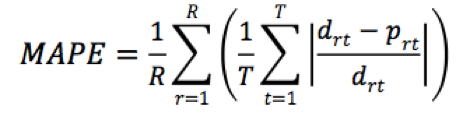
\includegraphics[width=0.2\textwidth]{MAPE.png}
  
  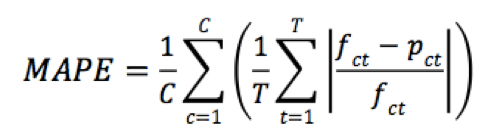
\includegraphics[width=0.2\textwidth]{MAPE-2.png}
  \caption{Evaluation Metrics}
  \captionsetup{justification=centering}
  \label{fig:18}
\end{figure}

\section{Conclusions}
\large
For this paper, we focus on solving the KDD-CUP 2017 the second task which is the traffic volume prediction. Traffic congestion is always a serious problem in big cities. It is good to provide traffic volume prediction model so that we can take action earlier which will save travel time, as well as reducing gas emission. We have easy entry level approach which is to calculate the average volume of 20 minutes interval. We found out that that is a really good strategy which leads us to rank 36 with MAPE 0.191 at the beginning. We use those list of volume number results as baseline to estimate the real MAPE which helps to develop advanced Decision Tree Model and advanced ARIMAX Time Series Model later for our research project. The result of Decision Tree model has the best over all MAPE 0.2298 and MAPE 0.288 for ARIMAX Time Series Model. We assume that those two results are over fitting the ground truth which make the MAPE worse. For the future work, we plan to keep turning the parameters of the Decision tree model and ARIMAX model to reduce the MAPE. Moreover, we will try to apply different Machine Learning Methodology such as Gaussian Linear Regression, AbaBoost Tree, Hidden Markov Model algorithm, etc.

\section{Appendix}
\large
\subsection{Milestone}
The table below shows the timeline for this project. We are going to follow our schedule to complete each milestone on time.
\begin{table}[ht]
%\caption{} % title of Table
\centering % used for centering table
\begin{tabular}{c| c| c} % centered columns (4 columns)
\hline\hline %inserts double horizontal lines
Date & Milestone & Description of Work  \\  % inserts table
%heading
\hline % inserts single horizontal line
Mar 15 & Proposal Complete & 2-3 Pages  \\ % inserting body of the table 
\hline
Mar 22 & Methodology For task-1 & Methodology Due  \\
\hline
Mar 29 & Training Result Due & Training Model  \\
\hline
April 05 & Evaluation Result Due & MAPE Result  \\  % [1ex] adds vertical space
\hline
April 12 & Training Result task-2 & Training Model \\
\hline
April 19 & Evaluation Result Due & MAPE Result \\
\hline
April 26 & Final Paper Presentation & Turn In \\
\hline %inserts single line
\end{tabular}
\label{table:nonlin} % is used to refer this table in the text
\end{table}

\subsection{Schedule}
We recorded the whole participation during the whole competition process, in order to summarize the pros and cons of different models and parameters we tried.
\begin{figure} [H]
  \centering
  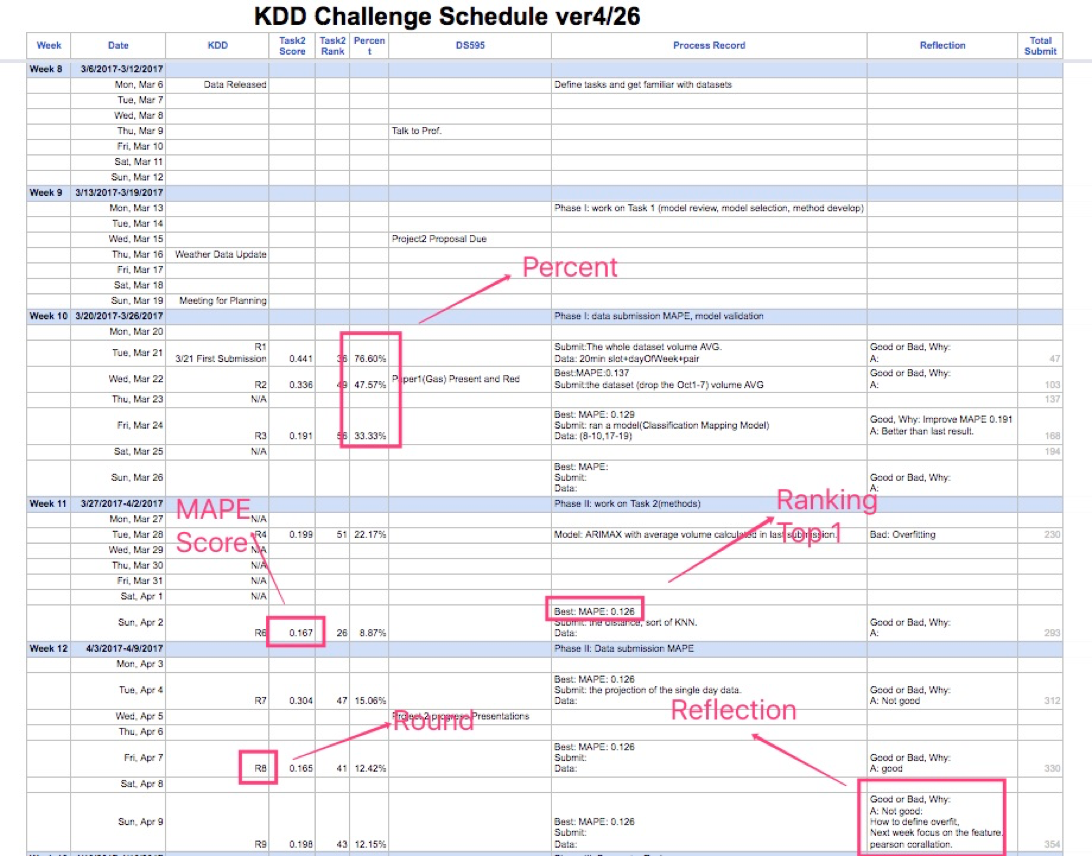
\includegraphics[width=0.49\textwidth]{kdd_schedule.png}
  \caption{Schedule}
  \label{fig:19}
\end{figure}

\begin{thebibliography}{99}
% \large 
\bibitem{c1}G. Wu, Y. Ding, Y. Li, J. Bao, Y. Zheng, and J. Luo, “Mining Spatio-Temporal Reachable Regions over Massive Trajectory Data,” pp. 1–12, Oct. 2016.
\bibitem{c2}Y. Ding, Y. Li, K. Deng, H. Tan, M. Yuan, and L. M. Ni, “Detecting and Analyzing Urban Regions with High Impact of Weather Change on Transport,” IEEE Transactions on Big Data, vol. PP, no. 99, pp. 1–1, 2016.
\bibitem{c3}Z. Liu-Hua, C. Shi-Dong, K. Ling-Jiang, and L. Mu-Ren, “The influence of tollbooths on highway traffic,” 2007.
\bibitem{c4}K. Komada and T. Nagatani, “Traffic flow through multi-lane tollbooths on a toll highway,” Physica A: Statistical Mechanics and its Applications, vol. 389, no. 11, pp. 2268–2279, Jun. 2010.
\bibitem{c5}Shi Fang, K. Bian, and K. Xie, “Vulnerability analysis of highway traffic networks using origin-destination tollgate data,” presented at the 2016 IEEE 19th International Conference on Intelligent Transportation Systems (ITSC), 2016, pp. 1957–1963.
\bibitem{c6}M. Tong and H. Xue, “Highway Traffic Volume Forecasting Based on Seasonal ARIMA Model,” Journal of Highway and Transportation Research and Development (English Edition), vol. 3, no. 2, pp. 109–112, Dec. 2008.
\bibitem{c7}L. Huang and M. Barth, “A Novel Loglinear Model for Freeway Travel Time Prediction,” presented at the 2008 11th International IEEE Conference on Intelligent Transportation Systems (ITSC), 2008, pp. 210–215.
\bibitem{c8}Y. Zhang and H. Ge, “Freeway Travel Time Prediction Using Takagi-Sugeno-Kang Fuzzy Neural Network,” Computer-Aided Civil and Infrastructure Engineering, vol. 28, no. 8, pp. 594–603, May 2013.
\bibitem{c9}W. Qiao, A. Haghani, C.-F. Shao, and J. Liu, “Freeway path travel time prediction based on heterogeneous traffic data through nonparametric model,” Journal of Intelligent Transportation Systems, vol. 20, no. 5, pp. 438–448, Sep. 2015.
\bibitem{c10}C.-S. Li and M.-C. Chen, “A data mining based approach for travel time prediction in freeway with non-recurrent congestion,” Neurocomputing, vol. 133, pp. 74–83, Jun. 2014.
\bibitem{c11}X. Xing, D. Yu, X. Tian, and Z. Cheng, “Freeway travel time prediction based on clustering method with data mining,” pp. 1–6, Sep. 2016.
\bibitem{c12}M. Tong and H. Xue, “Highway Traffic Volume Forecasting Based on Seasonal ARIMA Model,” Journal of Highway and Transportation Research and Development (English Edition), vol. 3, no. 2, pp. 109–112, Dec. 2008.
\bibitem{c13}J. Liu, L. Sun, W. Chen, and H. Xiong, “Rebalancing Bike Sharing Systems,” presented at the Proceedings of the 22nd ACM SIGKDD International Conference on Knowledge Discovery and Data Mining - KDD '16, 2016.

\bibitem{c14}'How did I get the Top 5\% on the Tianchi Challenge', https://zhuanlan.zhihu.com/p/23845169

\end{thebibliography}

\end{document}